\subsection{Hemmelig kommunikation før internettet}
I dette afsnit vil der blive kigget på, hvordan man tidligere har anvendt kryptografi i tiden inden internettets udbredelse, som skete i de sene 1980'ere. Dette vil gøres for at skabe en basal forståelse for hvordan kryptering, eller kryptografi, er blevet til den teknologi der kendes i dag.\\\\
\noindent
For at skabe klarhed over begrebet, er der brug for først at kigge på selve definitionen af kryptografi, og hvad dets formål er og har været gennem tiden. 
Kunsten at kryptografere vil sige, at skjule information ved at transformere sin besked ind i en forudbestemt algoritme.
Dette vil sige at kryptografering ikke blot handler om at skjule, eller hemmeliggøre et større budskab, men nærmere at transformere noget førhenværende forståeligt, til noget der kun kan forståes, ved brug af en bestemt metode.\cite{MeningOfCryptography}
\subsubsection{De Egyptiske hieroglyffer}
Grundet denne definition, kan man også argumentere for, at alle verdens forskellige sprogs bogstaver og tegn, enten har været, eller stadig er, en form for uforståelig kryptografi, og derfor skal man først kigge på det ældgamle Egypten, 1900 B.C. for at finde de ældste daterede tegn på, eller former for kryptografi.\cite{PastCryptography} Selv om man dog også kan diskutere hvorvidt der forefindes noget ældre, så som hulemændenes forskellige væg tegninger.
\begin{figure}[H]
    \centering
    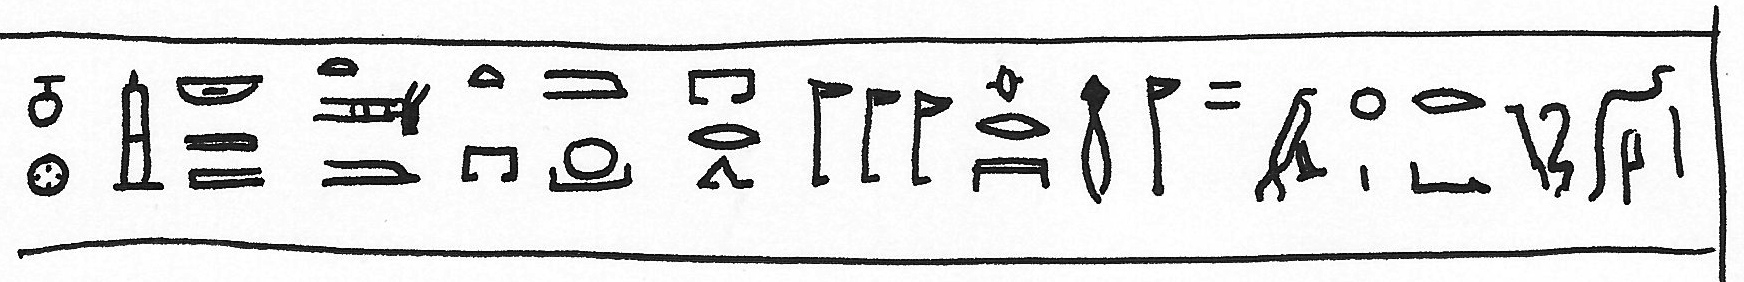
\includegraphics[width=0.8\textwidth, angle =0]{Projectdoc/Problemanalyse/Illustrationer/egypten.jpg}
    \caption{Egyptiske hieroglyffer}
    \label{fig:hieroglyffer}
\end{figure}
\noindent
Disse hieroglyffer siges nemlig at være menneskets første form for tekst, og må derfor i begyndelsen ikke have været for alle til at forstå. Som tiden udviklede sig, lærte det almene Egypten dog at tolke hieroglyffer, og denne første kryptografi, "De egyptiske hieroglyffer [Se Figur: \ref{fig:hieroglyffer}]", blev til et anerkendt sprog.
Herefter er de næste former for kryptografi selvfølgelig alle de andre sprog, som efterhånden dukkede op, og senere udbredte sig til, samt blev globalt accepteret hos, selvstændige nationer.\\
I takt med denne udbredelse, viste der sig et nyt behov for at kunne skjule sine beskeder for andre, der også kunne læse eller skrive ens eget sprog. Den første løsning på dette problem skal findes i årene omkring 500 B.C.\cite{PastCryptography}
\subsubsection{Den spartanske scytale}
\begin{figure}[H]
    \centering
    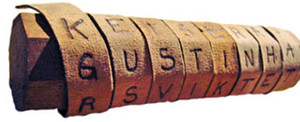
\includegraphics[scale=1.2]{Projectdoc/Problemanalyse/Illustrationer/scytale.jpg}
    \caption{En spartansk scytale}
    \label{fig:scytale}
\end{figure}
\noindent
Da det stadig i denne tid kun var de færreste, der kunne læse og skrive, betød det at de der faktisk kunne, reelt ikke havde den bedste forståelse for bogstavernes sammenhæng. Sammenlign lidt datidens forståelse af at kunne læse, som nutidens mindre børns niveau. Detfor kunne spartanerne opfinde en af de første former for kryptering, "Den Spartanske Scytale [Se Figur:\ref{fig:scytale}]". Denne spartanske scytale var en cylinder, hvorom man viklede noget at skrive på, herefter skrev man sin besked på de enkelte sider, således når man fjernede cylinderen kunne man ikke forstå sammenhængen, før man havde en cylinder i samme størrelse. Denne kryptering ville dog i dag ikke være særlig svær at dekryptere, og kendes også i flere former under begrebet bogstavstransponering.
\subsubsection{A-K kodens fødsel}
Den næste daterede form for kryptering findes allerede små 500 år efter, i det gamle Rom, regeret under Julius Caesar, og siges faktisk også at være opfundet af Julius Caesar ham selv.\cite{PastCryptography}\\ 
Det romerske militær havde brug for at skjule deres strategiske beskeder for fjenden, som ofte fangede de romerske budbringere, i forsøget på at danne et militærisk modtræk. Ceasar opfandt derfor, den største af de i nyere tids kendte kryptografiske metoder, kaldet bogstavs substitution eller "A-K Koden".\\
A-K Koden går i alt sin simpelhed ud på, at man flytter alfabetet en vis grad, f.eks. i A-K ville "ABCD" skrives "KLMN", eller i A-S ville "ABCD" skrives "STUV".\cite{TheSecretLanguage}
Som førnævnt er denne bogstavs substitution den mest udbredte og kendte kryptografiske metode, og er derfor også den mest udviklede. A-K Koden findes nemlig også i et utal af andre former.\\ 
F.eks. i formen af "Det hemmelig kodeords A-K", der udføres ved at først vælge et kodeord, "KODEORD", hvorefter kodeordets bogstaver flyttes til starten af alfabetet, for tilsidst at fortsættes resten af alfabetet, derfor ville "ABCDEFGHIJKLMNO" skrives "KODEORDABCFGHIJ", således at "HEJ" ville skrives "AOC". \cite{TheSecretLanguage}\\
For andre former af A-K Koden kunne nævnes "Alberti-Vigeneres Cipher" opfundet i midt 1400 tallet, "The Vingenere Cipher" fra 1500'erne, eller Jefferson's Wheel Cipher fra det sene 1700\cite{PastCryptography}, der alle som Caesar's koncept, fungerer ved udbytning af bokstavers rækkefølge, men dog i de nævnte også ved hjælp af et værktøj, som ved Den Spartanske Scytale.\\
\subsubsection{Den nyere tids kryptografi}
Faktisk er A-K Koden så anvendt at man skal helt frem til 1800 tallet, før der igen findes en ny og anderledes kryptografi. I 1836 blev den revolutionerende teknologi "Morse Kode" nemlig opfundet af Samuel Morse. Denne teknologi blev alment anvendt til at transmittere beskeder over telegrafens netledninger, også senere kendt som telefonnettet.\cite{Telegraphing}.\\
I de efterfølgende år i det tidlige 1900 tallet, kan man igen også finde flere former, både inden for nyopfundet og genopfundet kryptografering, da man grundet både den Første, og den Anden Verdens krig, havde lagt flere ressourcer til forskning i hemmeliggørelse af beskeder. Blandt andet var det også i denne tid, at den kendte enigma krypteringsmaskine blev opfundet.\cite{PastCryptography}
\begin{figure}[H]
    \begin{subfigure}{0.5\textwidth}
    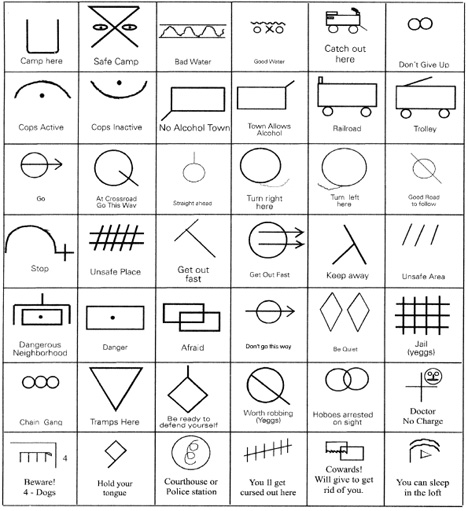
\includegraphics[width=0.9\linewidth, height=5cm]{Projectdoc/Problemanalyse/Illustrationer/hobo-glyphs-code.jpg} 
    \caption{The Hobo Code}
    \label{fig:hobocode}
    \end{subfigure}
    \begin{subfigure}{0.5\textwidth}
    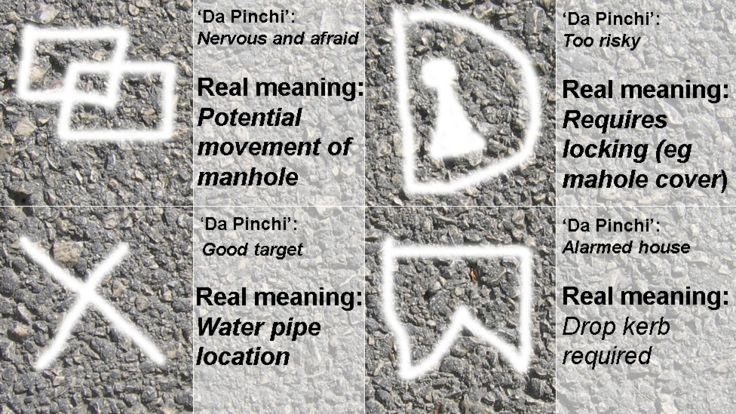
\includegraphics[width=0.9\linewidth, height=5cm]{Projectdoc/Problemanalyse/Illustrationer/BurglarsCode.jpg}
    \caption{Da Pinchi Code / The Burglars Code}
    \label{fig:burglarscode}
    \end{subfigure}
    \caption{To af de legendariske kryptografi metoder}
    \label{fig:legendscode}
\end{figure}
\noindent
Foruden alle disse førnævnte daterede og kendte former for kryptografi, kan man selvfølgelig også finde en lang række af ikke daterede, eller ligefrem legendariske kryptografi metoder. Disse kan blandt andet have været anvendt både til handel, men også af f.eks. hjemløse.\\
Et kendt eksempel på dette kunne være "The Hobo Code [Se Figur: \ref{fig:hobocode}]", en bestemt form for kryptografi kendt, og anvendt af hjemløse til at hjælpe hinanden med deres overlevelse\cite{TheHoboCode}. Disse beskeder var aldrig rigtigt blevet dateret, og derfor kender ingen deres præcise oprindelse, men det vides dog at denne kryptografi har været anvendt i flere århundrede. Derud over vides også at der findes flere andre afarter af denne kendte kode, såsom den nytidiske "Da Pinchi Code [Se Figur: \ref{fig:burglarscode}]", anvendt af konstruktions arbejdere, eller efter historier også af indbrudstyve.\cite{DaPinchiCode}\\
Tilsidst i det sene 1900 blev internettet opfundet, og siden da har kryptografi for det meste været anvendt i forskellige former til beskyttelse af data på computere, så som hash algoritmer.
